\documentclass[11pt,a4paper]{article}
\usepackage[left=2cm,right=2cm,top=2cm,bottom=3cm]{geometry}
\usepackage{amsmath,amsfonts,amsthm,amssymb,varioref,times, commath}
\usepackage{gensymb}
\usepackage{tikz}
\usepackage{textcomp}
\usepackage{hyperref}
\hypersetup{
 colorlinks=true,
 linkcolor=blue,
 filecolor=magenta, 
urlcolor=cyan,
}
\usepackage{lipsum}
\usepackage{epigraph}
%to resume numbering in a list
\usepackage{enumitem}
%----- arrows 
\usepackage{extarrows}

%    differential equatiosn 
\usepackage{diffcoeff}   %\diff[2]{x}{y}


%%%%%%pour ecrire en français avec les accents
\usepackage[utf8]{inputenc}
\usepackage[T1]{fontenc}
\usepackage{lmodern} % load a font with all the characters
\usepackage{units}
%%%%%%%Image-related packages
\usepackage{wrapfig}
\usepackage{float, graphicx}
\graphicspath{ {./img/} }
\usepackage{subcaption}
\usepackage[export]{adjustbox}

%%%%%%%pour faire des cadres
\usepackage{xcolor}
\usepackage{tcolorbox}
\usepackage{framed}
\usepackage{mdframed}


%%%%%%%chemistry frmulae
\usepackage{chemfig}
\usepackage{chemformula}
\usepackage[version=4]{mhchem}

% -------------- Circuits -------------------
\usepackage[european, straightvoltages]{circuitikz}

% Title & headers
\usepackage[explicit]{titlesec}
% Raised Rule Command:
% Arg 1 (Optional) - How high to raise the rule
% Arg 2 - Thickness of the rule
\newcommand{\raisedrulefill}[2][0ex]{\leaders\hbox{\rule[#1]{1pt}{#2}}\hfill}
\titleformat{\section}{\Large\bfseries}{\thesection. }{0em}{#1\,\raisedrulefill[0.4ex]{1pt}}

% pour ecrire sur +sieurs colonnes
\usepackage{multicol}
\setlength{\columnseprule}{0pt}
\setlength{\columnsep}{60pt}
% Fusion de lignes de tableaux.
\usepackage{multirow}
% Position verticale des lettres dans la ligne de tableau.
\usepackage{array}

% physics -----------------------------------------------------------
\newcommand{\To}{\longrightarrow}
\newcommand{\gpl}{\; g\cdot L^{-1}}
\newcommand{\gpmol}{\; g\cdot mol^{-1}}
\newcommand{\mpl}{\; mol\cdot L^{-1}}
\newcommand{\mps}{\; m\cdot s^{-1}}
\newcommand{\rps}{\; rad\cdot s^{-1}}
\newcommand{\kph}{\; km\cdot h^{-1}}
\newcommand{\mpss}{\; m\cdot s^{-2}}
\newcommand{\Dt}{\Delta t}
\newcommand{\vv}{\vec{v}}
\newcommand{\va}{\vec{a}}
\newcommand{\vp}{\vec{p}}
\newcommand{\vf}{\vec{F}}
\newcommand*{\Vf}[1]{\overrightarrow{F_\ensuremath{{#1}}}}
\newcommand{\es}[1]{\cdot10^{#1}}
\newcommand{\eng}[1]{\textcolor{purple}{(= #1})}
\usepackage{harpoon}
%\newcommand*{\vect}[1]{\overrightharp{\ensuremath{#1}}}
\newcommand*{\Vect}[1]{\overrightarrow{\ensuremath{#1}}}
\newcommand{\pfd}[1]{\sum \vec{F}_{ext_{#1}} &= \od{\vp_{#1}}{t} = m\cdot\va_{#1}}
\newcommand{\C}{\degree C}
\newcommand{\Delt}{\Delta t}

% --- Circuits ------------
\newcommand{\bipole}[1]{
\begin{circuitikz} \draw
(0,0) to[ #1 ] (2,0); 
\end{circuitikz} {\hspace{5mm}}}

% Chimie ---------------------------------
\newcommand{\oxo}{\ce{H3O+}_{(aq)}}
\newcommand{\eau}{\ce{H2O}_{(\ell)}}
\newcommand{\OH}{\ce{HO-}_{(aq)}}
\newcommand{\AH}{\ce{AH}_{(aq)}}
\newcommand{\A}{\ce{A-}_{(aq)}}
\newcommand{\MnO}{\ce{MnO_4^{-}}}
\newcommand{\conc}[1]{\left[{#1}\right]}
\newcommand{\couple}[2]{\ce{#1/#2}}


% Environnements ------------------------
\newcounter{exo}
\newenvironment{exo}[1][]
{\refstepcounter{exo} \begin{shaded}\noindent $\triangleright \quad$\textbf{Exercice~\theexo. #1} } { \end{shaded}}
\newenvironment{eg}
{\begin{shaded} \textbf{Exemple:} } { \end{shaded}}

\newenvironment{defn}[1]
{\begin{leftbar}\noindent \textbf{Définition :\textit{ \quad #1}} } { \end{leftbar}}

%\newenvironment{rmrq}
%{\begin{shaded} \textbf{Remarque.\quad } \itshape } { \end{shaded}}
\newenvironment{rmrq}
{\begin{mdframed}[backgroundcolor=blue!10, linewidth=0pt] \textbf{Remarque.\quad } \itshape } { \end{mdframed}}

\newenvironment{python}
{\begin{shaded} \textbf{A faire en PYTHON}\\ \itshape } { \end{shaded}}

% Shading colour -----------------------------
\definecolor{shadecolor}{gray}{0.9}

\date{}
\author{}

\renewcommand*\contentsname{Résumé}









% parametres des entete et de pieds de pages
\usepackage{fancyhdr}
\pagestyle{fancy}
\fancyhf{}
\lhead{SciPhy : Terminale spé}
\rhead{Ch. 2 : équilibre chimique}
\chead{2020-28}
\rfoot{Page \thepage}
\lfoot{\textcopyright\; S Zayyani}


\title{\large Chimie - Chapitre 2 \\ \LARGE  Les réactions limitées : l'équilibre chimique \\}

\setlength{\parindent}{0mm}
\setlength{\parskip}{2mm}

%%%%%%%%%%% For wrapfigure 
\setlength{\intextsep}{6pt}%
\setlength{\columnsep}{3pt}%


\begin{document}
\maketitle
\vspace{-1cm}

\begin{tcolorbox}[title=Notions de la classe de première à rappeler]
Tableaux d'avancement ; avancement chimique ; Concentration molaire
%\tcblower
\end{tcolorbox}
\tableofcontents

\section{Transformations totales \& limitées}

On considère qu’une réaction chimique est à l’état final (i.e. terminée) lorsque les quantités de matière des différentes espèces chimiques n’évoluent plus.  A l’état final l’avancement final de la réaction est noté $x_f$ .  Si à l’état final un des réactifs est totalement épuisé, l’avancement atteint alors sa valeur maximale, notée $x_{max}$.  

\begin{defn}{Réaction totale \& limitée}
\begin{itemize}
    \item Une transformation chimique est \textbf{totale} si le réactif limitant a entièrement disparu à l’état final.  L’avancement final est donc égal à l’avancement maximal. \[ x_f = x_{max} \]
    \item Une transformation chimique est limitée si le réactif limitant n’a pas totalement disparu à l’état final.  L’avancement final est donc inférieur à l’avancement maximal : \[ x_f < x_{max} \]
	\item Le \textbf{taux d’avancement} final $\tau$ d’une réaction chimique est : \[ \tau = \dfrac{x_f}{x_{max}} \]
	Si $ \tau \approx 1$ la transformation est totale ; si $\tau < 1$ la transformation est limitée. 
\end{itemize}
\end{defn}

\section{Équilibre chimique}

\begin{defn}{Équilibre chimique}
\begin{itemize}
    \item Un système chimique, siège d’une transformation limitée, est dans un état d’équilibre chimique à la température $T$ et pression $P$, lorsque les \textbf{concentrations des réactifs et des produits n’évoluent plus}.  
    \item Cet état correspond à l’\textbf{état final de la transformation}.  
    \item Il s'agit d'un \textbf{équilibre dynamique}, c’est-à-dire il ne se traduit pas par l’absence de réaction chimique, mais par la \textbf{coexistence de deux réactions inverses se produisant simultanément et à la même vitesse}. 
    \item Les deux réactions sont $\quad A+B\longrightarrow C + D \quad $, la réaction ``directe''; et $\quad  C + D \longrightarrow A + B \quad $, la réaction ``inverse''.
    \item Si la réaction directe et la réaction inverse ont lieu \textbf{à la même vitesse}, alors, la réaction étudiée est en équilibre. 
    \item Afin de représenter cet état d’équilibre nous utilisons une double-flèche ``$\rightleftharpoons$'' (ou parfois ``='' même ce signe est réservé plutôt pour les demi-équations rédox ou acidobasiques) au lieu d'une flèche simple $\righttarrow$. En prenant donc l’exemple du cas précédent : \[ A + B \rightleftharpoons C + D \]
\end{itemize}
\end{defn}

Il est important donc de noter que désormais la \textbf{flèche simple est utilisée exclusivement dans le cas d'une réaction totale} (car dans ce cas, il n’y a plus la réaction inverse). 

En réalité, même dans le cas des réactions totales, il y a toujours une réaction inverse, mais la vitesse de cette réactions est tellement faible devant le sens direct que la réaction globale est presque totalement dans le sens direct. 


\section{Constante d'équilibre d'une réaction}

\begin{defn}{Quotient de réaction}
\begin{itemize}
    \item Considérons le système chimique suivant : \[aA_{(aq)} + bB_{(aq)} \rightleftharpoons cD_{(aq)} + dD_{(aq)}\]
    À un instant donné de l'évolution du système chimique, le quotient de la réaction est défini par  
    \[
    Q_r = \dfrac{\left[C\right]^c\cdot\left[D\right]^d}{\left[A\right]^a\cdot\left[B\right]^b}
    \]
    \item Le quotient de réaction $Q_r$  est sans unité, et $[X]$  signifie la valeur numérique de la concentration (en $\mpl$ l’espèce $X$ dans la solution).
\end{itemize}
\end{defn}

\begin{rmrq}
Même quand il est le réactif ou le produit d’une réaction, le \textbf{solvant} (presque toujours eau) est représenté dans le quotient de réaction par le chiffre $1$.

Dans le cas d’une transformation mettant en jeu des \textbf{solides} en tant que réactif ou produit, ces solides sont représentés dans le quotient par le chiffre $1$.
\end{rmrq}

\begin{exo}
\begin{enumerate}
    \item Quelle est la signification d'un quotient de $Q_r = 0$? 
    \vspace{.5cm}
    \item Quel serait le coefficient de réaction d’une réaction totale ? et pourquoi?
    \vspace{.5cm}
    \item Considérer la réaction suivante, avec $K = 2,7\es{3}$ : $\ce{Ni}_{(s)} + \ce{Pb^2+_{(aq)} \rightleftharpoons \ce{Ni^2+_{(aq)}} + \ce{Pb_{(s)}}}$
    
    Dans l'état initial, un bécher contient une lame de nickel, une lame de plomb, des ions de nickel de concentration $[\ce{Ni^2+}]_i=1,0 \mpl$ et des ions plomb de concentration $[\ce{Pb^2+}]_i=2,0\es{-4}\mpl$. 
    
    Calculer le quotient de la réaction, et déterminer le sens de l'évolution spontanée du système. 
    \vspace{2cm}
\end{enumerate} 
\end{exo}	 
 
\begin{exo}
Un système chimique de volume $V = 20\; mL$, constitué initialement de $2,0\es{-4}\; mol$ d'ions iodure, et de $5,0\es{-5}\; mol $ d'ion peroxodisulfate \ce{ S2O8^2- }, est le siège d'une transformation lente et totale d'équation chimique : 
\[ 2\;\ce{I-}_{(aq)} + \ce{S2O8^2- }_{(aq)} \To \ce{I2}_{(aq)} + 2\;\ce{SO4^2- }_{(aq)}
\] 
\begin{enumerate}
    \item Donner l'expression littérale du quotient de la réaction. 
    \item Exprimer les concentrations des réactifs et des produits en fonction de l'avancement $x$ et de leurs quantités initiales. En déduire l'expression de $Q_r$  en fonction de $x$. 
    \item Calculer $Q_{r,i}$ le quotient de réaction initial, et $Q_{r,1/2}$ sachant qu'au temps de demi-réaction $x_{1/2}=2,5\es{-5}\; mol$.
\end{enumerate}
\textbf{Solution : }

\begin{enumerate}
    \item $ Q_r = \dfrac{\left[\ce{I2}\right]\cdot\left[\ce{SO4^2- }\right]^2}{\left[\ce{I-}\right]^2\cdot\left[\ce{S2O8^2- }\right]} $
    \item d'après le tableau d'avancement on peut déterminer : 
    \begin{align*}
        \left[\ce{I2}\right] &= \dfrac{x}{V} \\
        \left[\ce{SO4^2- }\right] &= \dfrac{2x}{V} \\
        \left[\ce{S2O8^2- }\right] &= \dfrac{\Big( n_i(\ce{S2O8^2- }) - x\Big)}{V}       \\
        \left[\ce{I- }\right] &= \dfrac{ \Big( n_i(\ce{I- }) - 2x\Big)}{V}
    \end{align*}
    et donc le quotient de la réaction : $Q_r = \dfrac{4x^3}{\Big( n_i(\ce{I- }) - 2x\Big)^2\cdot \Big( n_i(\ce{S2O8^2- }) - x\Big)}$
    \item À l'état initial : $x=0$ et donc $Q_{r,i} = 0$
    
    Au temps de demi-réaction : $Q_{r,1/2} = 0,11$. 
\end{enumerate}
\end{exo}

\begin{defn}{Constante d'équilibre d'une réaction}
\begin{itemize}
    \item À chaque équation d’une réaction chimique (limitée) est associée une grandeur, la \textbf{constante d’équilibre}, notée $K$.  
    \item La constante d'équilibre correspond au \textbf{quotient de réaction à l'équilibre}, noté $Q_{r,éq}$, c'est-à-dire : 
        \[
    Q_{r,éq} = K = \dfrac{\left[C\right]^c_{éq}\cdot\left[D\right]^d_{éq}}{\left[A\right]^a_{éq}\cdot\left[B\right]^b_{éq}}
    \]
    \item À l'équilibre, donc, $Q_r = K$ tandis que en dehors de l’équilibre $Q_r \neq K$
    \item Il est important de comprendre que \textbf{$K$ est une constante}, et que \textbf{sa valeur ne dépend pas de la concentration initiale des réactifs}, car $Q_{r,eq}$  ne dépend que de la réaction chimique considérée et de la température. 
\end{itemize}
\end{defn}

\begin{rmrq}
Le quotient de réaction permet de caractériser l'état d'avancement d'une réaction, et ainsi de prévoir son évolution. Il s'agit donc d'une grandeur variable. La constante d'équilibre $K$ est bien une constante, il s'agit d'une propriété de la réaction en question, une constante qui caractérise la nature totale ou limitée de la réaction. 

De plus, nous pouvons prévoir le sens de la réaction en comparant la valeur de $Q_r$ à la valeur de $K$ c'est-à-dire $Q_{r,éq}$.  La réaction va avancer dans le sens où $Q_r$  évoluera vers $K$. 
\end{rmrq}

\centering
\section{Exercices Résolus}
\begin{figure}[h]
    \centering
    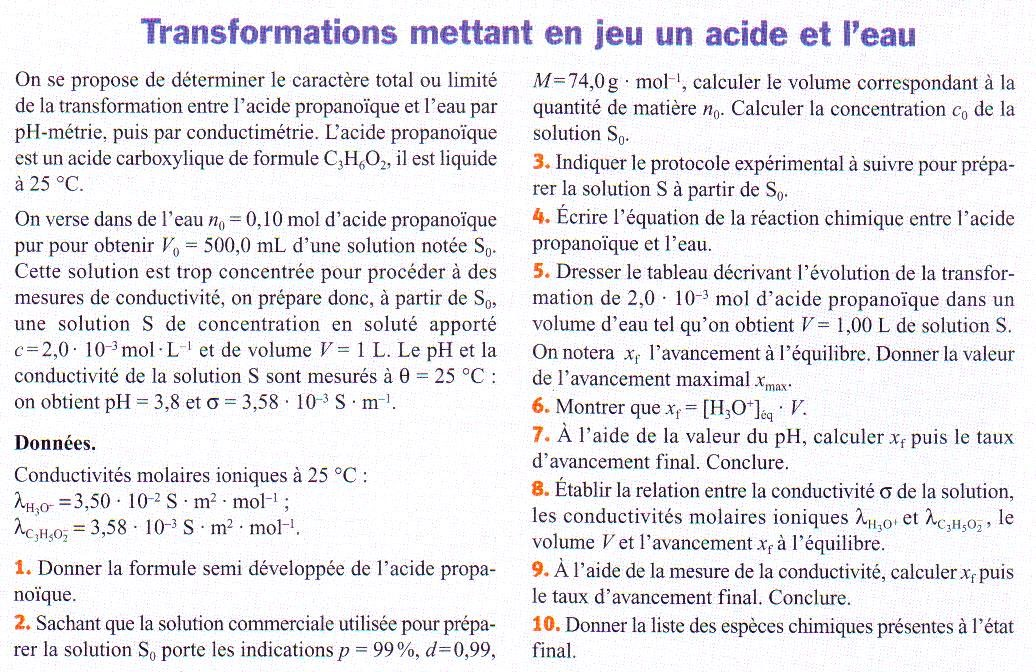
\includegraphics[width=\linewidth]{imgs/c2/xo1.jpg}
\end{figure}

\begin{figure}[h]
    \centering
    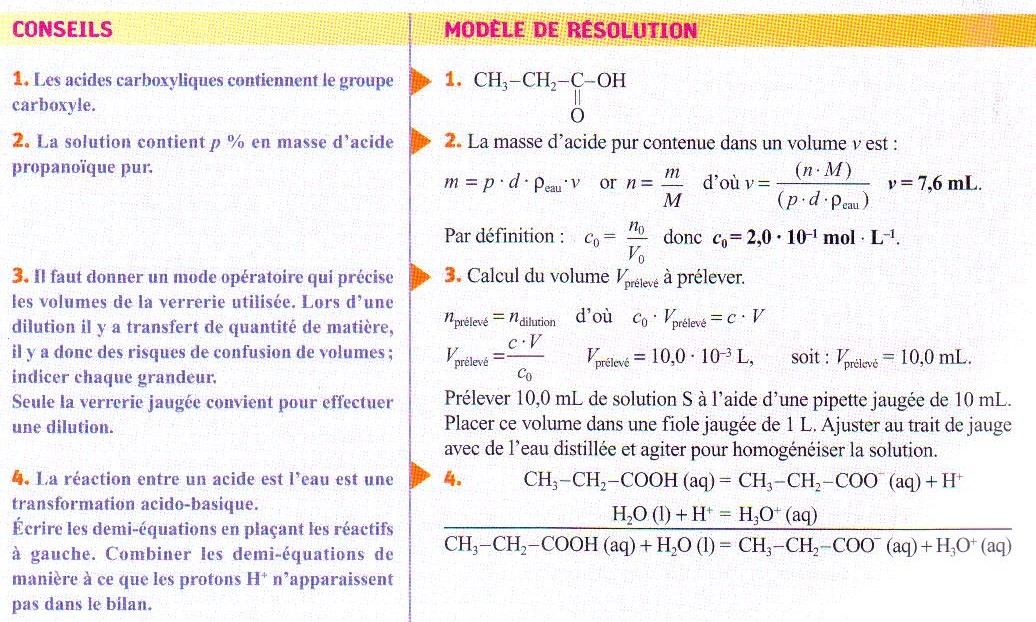
\includegraphics[width=0.9\linewidth]{imgs/c2/cxo1.jpg}
\end{figure}
\begin{figure}[h]
    \centering
    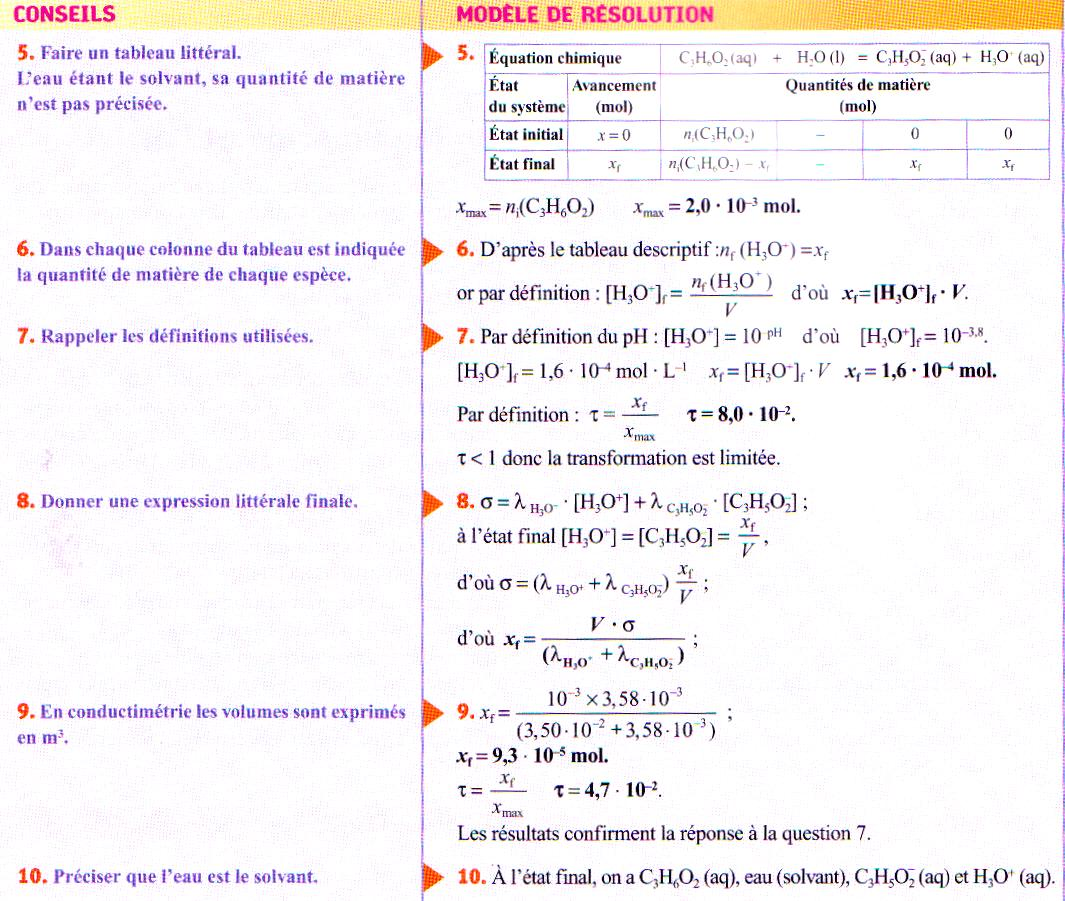
\includegraphics[width=0.9\linewidth]{imgs/c2/cxo1a.jpg}
\end{figure}






\end{document}
